\chapter{Diagnóstico}

Neste capítulo são apresentados o estado atual de trabalho da equipe, o estado desejado e as recomendações estabelecidas
a partir do diagnóstico realizado.

\section{Estado Atual}

Observando o estado atual da equipe foram identificados os seguintes pontos:

\begin{itemize}
  \item Utilização da metodologia ágil Scrum;
  \item Processo imaturo;
  \item Não está devidamente formalizado;
  \item Pouco medido e controlado;
  \item Riscos tratados de forma reativa.
\end{itemize}

Afim de identificar como a equipe trabalha foi feito um esboço do processo atual que não está formalizado. Seu objetivo é estabelecer
as atividades de análise de requisitos, construção e implantação do incremento de software. Este processo pode ser visto na 
Figura \ref{fig:processo_atual} e o seu detalhamento encontra-se no Apêndice \ref{ap:processo_atual}.


\begin{figure}[!ht]
\centering
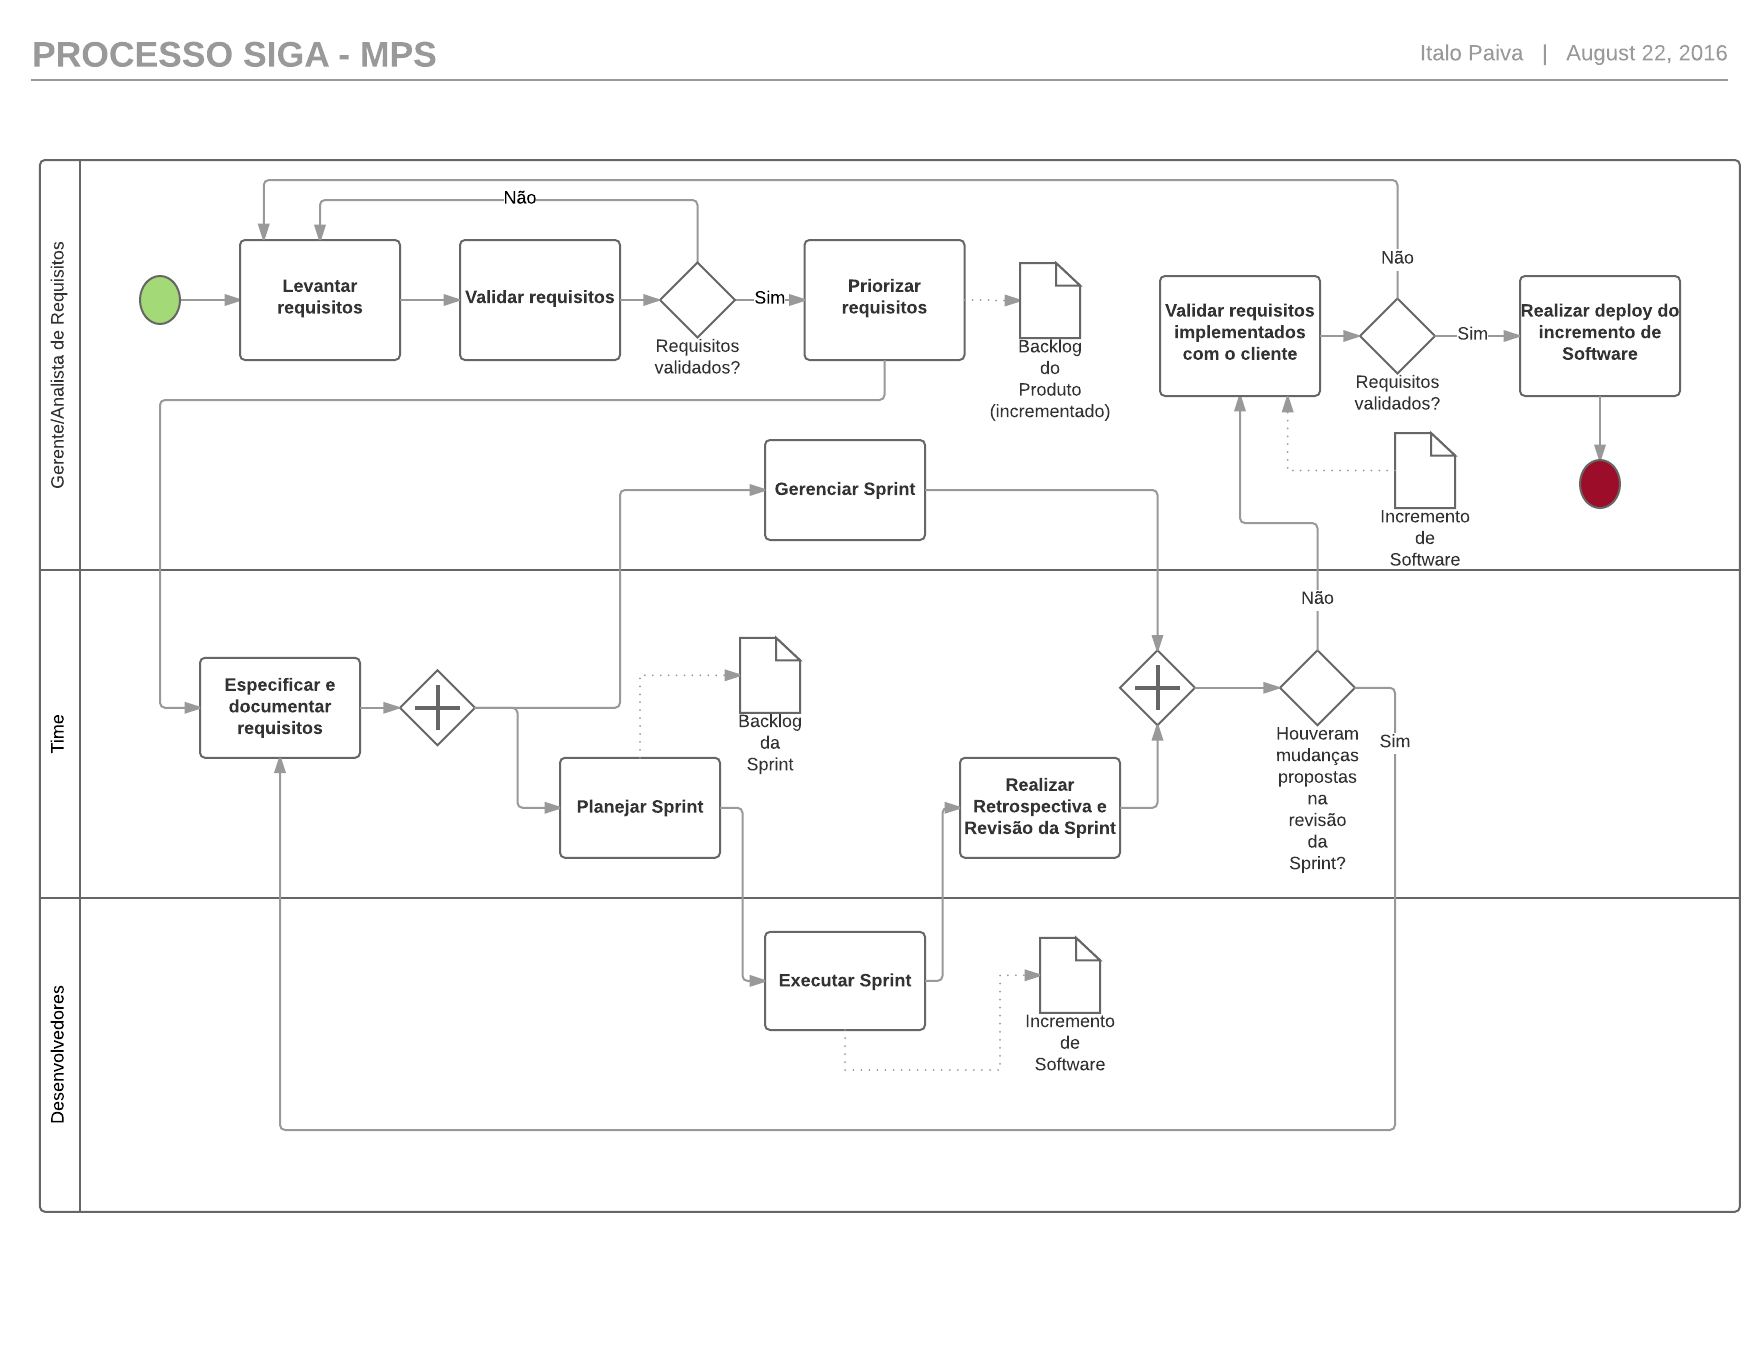
\includegraphics[scale=0.5]{figuras/processo_atual.png}
\caption{Processo Atual}
\label{fig:processo_atual}
\end{figure}

\section{Estado Desejado}

Após a execução desse projeto é esperado que haja uma melhoria do processo apresentado na Figura \ref{fig:processo_atual}, 
considerando principalmente aspectos gerenciais e de qualidade. Também é esperado que este processo seja formalizado e utilizado
de fato pela equipe. Dessa forma, o estado desejado pode ser sumarizado nos seguintes itens:

\begin{itemize}
	\item Processo de desenvolvimento de software formalizado;
  \item Execução das atividades do processo padronizadas;
	\item Execução das atividades do processo padronizadas;
	\item Processo minimamente medido e controlado.

\end{itemize}

	
\section{Recomendações}

A fim de alcançar o estado desejado foram estabelecidas algumas recomendações, são elas: 

\begin{itemize}
    \item Adicionar atividades de testes bem definidas no processo;
    \item Adicionar integração contínua no processo.
\end{itemize}
